\begin{frame}
	\centering \LARGE \color{naranjaUCA} Procesos de nacimientos y muerte
\end{frame}

\begin{frame}{Procesos de nacimientos y muerte}
	\begin{center}
		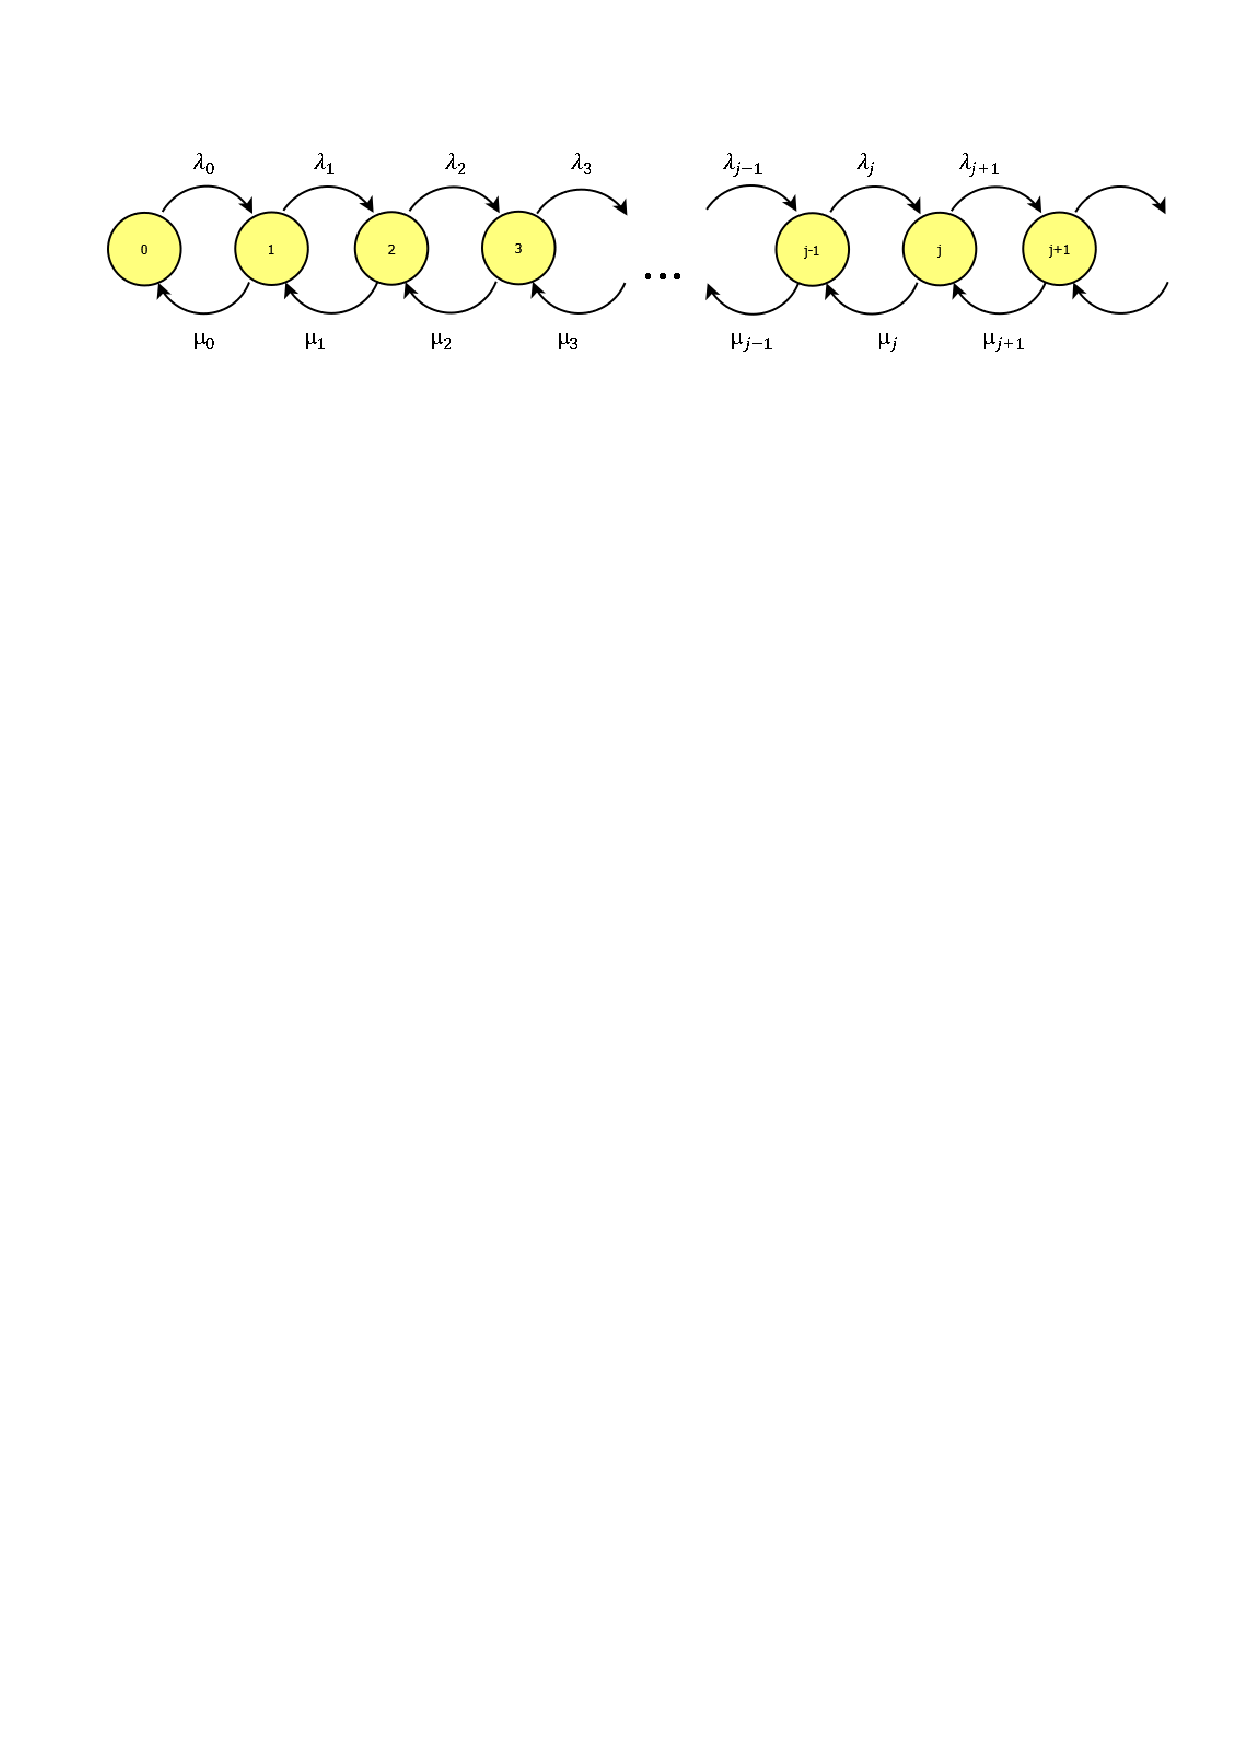
\includegraphics[trim = 10mm 220mm 10mm 25mm, clip,width=0.9\linewidth]{diagramatasa}
	\end{center}
	\pause
	Consideramos $p_{ij}^n$ la probabilidad de que, habiendo $i$ personas en el sistema, después de $n$ pasos haya $j$ personas. \\
	A partir de ahora supondremos que estamos en un estado estable.

\end{frame}
\begin{frame}{Leyes de movimientos}
	\begin{itemize}
		
		\item $P$(1 nacimiento entre $(t, t+h)$)=$\lambda_j h +o(h)$.\\
		El estado se incrementa en 1, esto es, $X(t+h)=j+1$.

		\item $P$(1 muerte entre $(t, t+h)$)=$\mu_j h +o(h)$.\\
		El estado se disminuye en 1, esto es, $X(t+h)=j-1$.
		
		\item Los nacimientos y muertes son independientes.
		
		
	\end{itemize} 

\end{frame}

\begin{frame}{Cáculo $\pi_{ij}$}
	Para $h$ pequeña: \pause
	
	\begin{equation*}
	\begin{split}
	p_{ij}(t+h)= p_{i,j-1}(t)P(\textrm{1 nacimiento en } (t,t+h))+\\
	+ p_{i,j+1}(t)P(\textrm{1 muerte en }(t,t+h))+\\
	+ p_{ij}(t)P(\textrm{ningún nacimiento ni muerte en }(t,t+h))
	\end{split}
	\end{equation*}
	\pause
	
	\begin{equation*}
	\begin{split}
	p_{ij}(t+h)= p_{i,j-1}(t)(\lambda_{j-1}h + o(h))+\\
	+ p_{i,j+1}(t)(\mu_{j+1}h + o(h))+\\
	+ p_{ij}(t)(1-\lambda_{j}h - \mu_{j}h + o(h) )
	\end{split}
	\end{equation*}
	
\end{frame}

\begin{frame}
	Reagrupando, diviendo entre $h$, tomando límite cuando $h \longrightarrow 0$:
	\pause
	\begin{equation*}
	p_{ij}'(t)= \lambda_{j-1} p_{i,j-1}(t) + \mu_{j+1}  p_{i,j+1}(t) - \lambda_j  p_{ij}(t) - \mu_{j} p_{ij}(t)
	\end{equation*}
	\pause
	Sustituyendo ahora las probabilidades de estado estable y reagrupando:
	\pause
	\begin{equation*}
	\lambda_{j-1} \pi_{j-1} + \mu_{j+1}  \pi_{j+1} = \pi_j(\lambda_j + \mu_j) \qquad (j= 1,2,...) \label{eq1}
	\end{equation*} 
	\pause
	Para $j=0$
	\pause
	\begin{block}{Ecuaciones de balance de flujo}
		\begin{equation*}
		\mu_1 \pi_1 = \pi_0 \lambda_0
		\label{eq2}
		\end{equation*}
	\end{block}
\end{frame}

\begin{frame}{Cálculo de los $\pi_{ij}$}
	Utilizando las hecuaciones de valance
\end{frame}

\begin{frame}{Cálculo de los $\pi_{ij}$}
	Utilizando las ecuaciones de balance 
	\begin{equation*}
	\pi_1=\frac{\pi_0 \lambda_0}{\mu_1}
	\label{eq3}
	\end{equation*}
	
	\pause
	Al sustituirlo en las ecuaciones de balance: para $j=1$ y despejando $\pi_2$ tenemos
	
	\begin{equation*}
	\pi_2=\frac{\pi_0(\lambda_0 \lambda_1)}{\mu_1 \mu_2}
	\label{eq4}
	\end{equation*}
	
	\pause
	Procediendo análogamente para $j=3,4,..$ se tiene que
	
	\begin{equation*}
	\pi_j=\pi_0 c_j
	\label{eq5}
	\end{equation*}
	
	$c_j=\dfrac{\lambda_0 \lambda_1 \cdots \lambda_{j-1}}{\mu_1 \mu_2 \cdots \mu_j}$
\end{frame}

\begin{frame}{Cálculo de los $\pi_{ij}$}
	Usando que \begin{equation*}
	\sum_{j=0}^{\infty}\pi_j=1 
	\label{eq6}
	\end{equation*}
	
	\pause
	Tenemos:
	\begin{equation*}
	\pi_0=\dfrac{1}{1+\sum_{j=1}^{\infty} c_j}
	\label{eq6}
	\end{equation*}
	\pause
	Se puede demostrar que si:
	$$
	\sum_{j=1}^{\infty} c_j = \infty $$
	Entonces el sistema no existe una distribución de estado estable.
\end{frame}
